


\documentclass[14pt]{report}

\usepackage{url,amssymb, amsmath,color}

\usepackage{fontspec}                     %加這個就可以設定字體                  %直接設定Windows中的字型,名字要打的一模一樣才行。
\XeTeXlinebreaklocale "zh"                %這兩行一定要加,中文才能自動換行
\XeTeXlinebreakskip = 0pt plus 1pt   

\usepackage{graphicx}


\title{\Huge Pattern Recognition}
\author{\huge Homework 2  \\ \\王淮慕\\學號 : 606415050\\系所 : 電機系}
\date{\today}
\begin{document}
	
	\maketitle
	
	\section{Find the maximum likelihood estimate of $ \theta $}
	\begin{enumerate}
		\item[Ans:] 
		\[p(x|\theta)=\frac{\theta^xe^{-\theta}}{x!},\quad x=0,1,2... \]
		\[p(D|\theta)=\prod_{k=1}^n p(x_k|\theta) \]
		\[l(\theta)=\ln P(D|\theta)=\sum_{k=1}^{n}p(x_k|\theta) \]
		\[\frac{\partial}{\partial \theta}l(\theta)=0\]
		\[\frac{\partial l(\theta)}{\partial \theta}=\frac{1}{\sum\limits_{k=1}^{n}k!}[\frac{(n+1)n}{2}\theta^{\frac{n^2+n-2}{2}}e^{-\theta n}+\theta^{\frac{n^2+n}{2}}(-n)e^{-\theta n}]=0 \]
		\[=\frac{1}{\sum\limits_{k=1}^{n}k!}(\frac{(n+1)n}{2\theta}-n)\theta^{\frac{n^2+n}{2}}e^{-\theta n}=0 \] 
		\[\frac{(n+1)n}{2\theta}=n \]
		\[\frac{n+1}{2}=\theta \]
		
	\end{enumerate}
	\section{Recursive Bayes Learning}
	\begin{enumerate}
		\item [(a)]Calculate and plot the posterior densities  $p(\theta |D^1)\ ,p(\theta |D^2)\ ,p(\theta |D^3)\ ,and\ p(\theta |D^4)\ $\\
		Ans :\\
		\[P(\theta|D^0)=p(\theta)=U(0,10) \]
		\[p(\theta | D^n)=\frac{p(x_n|\theta)p(\theta|D^{n-1})}{\int p(x_n|\theta)p(\theta|D^{n-1})d\theta} \]
			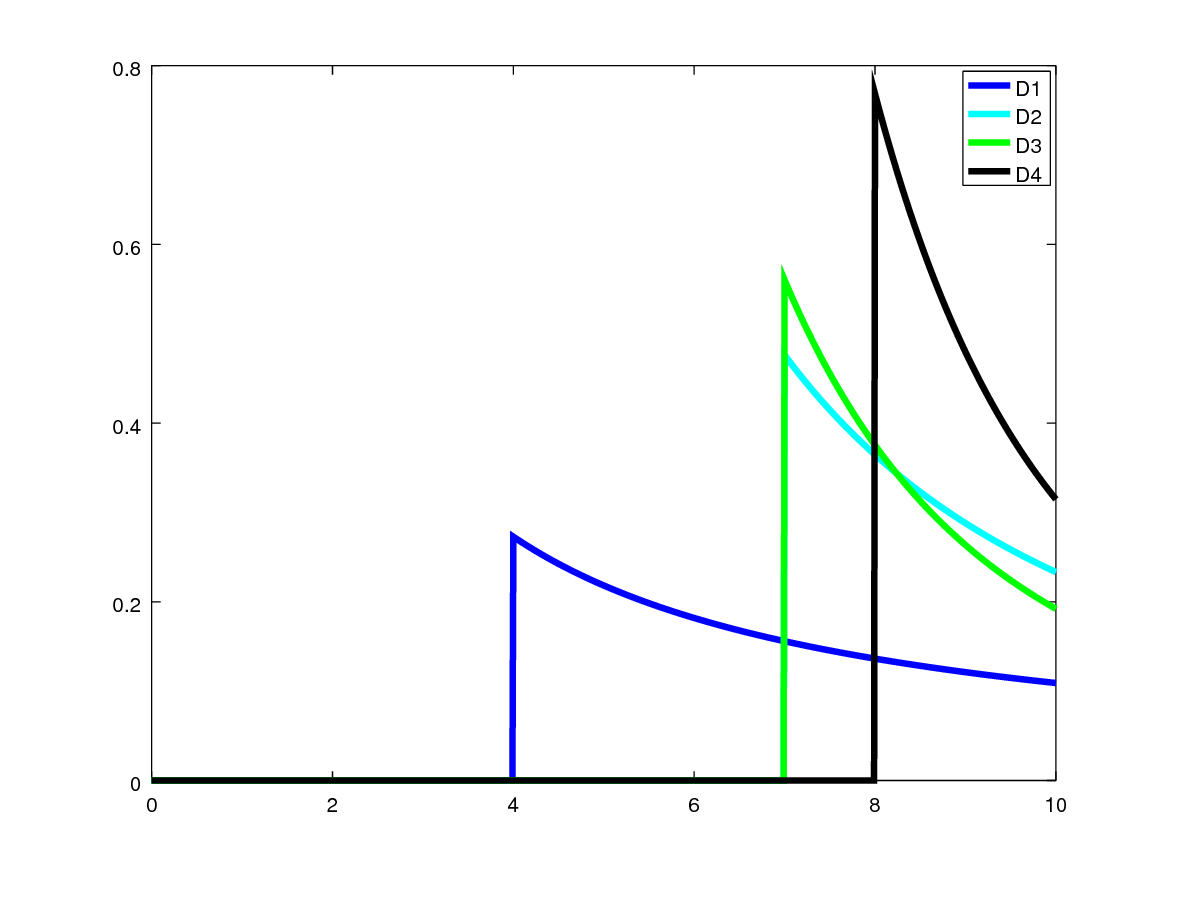
\includegraphics[width=0.5\textheight]{Question2_1.png}
		\item[(b)]Calculate and plot the desired density  $p(\theta |D^4)$ \\
		Ans : \\
		\[p(x|D)=\int p(x|\theta)p(\theta|D)d\theta \]
			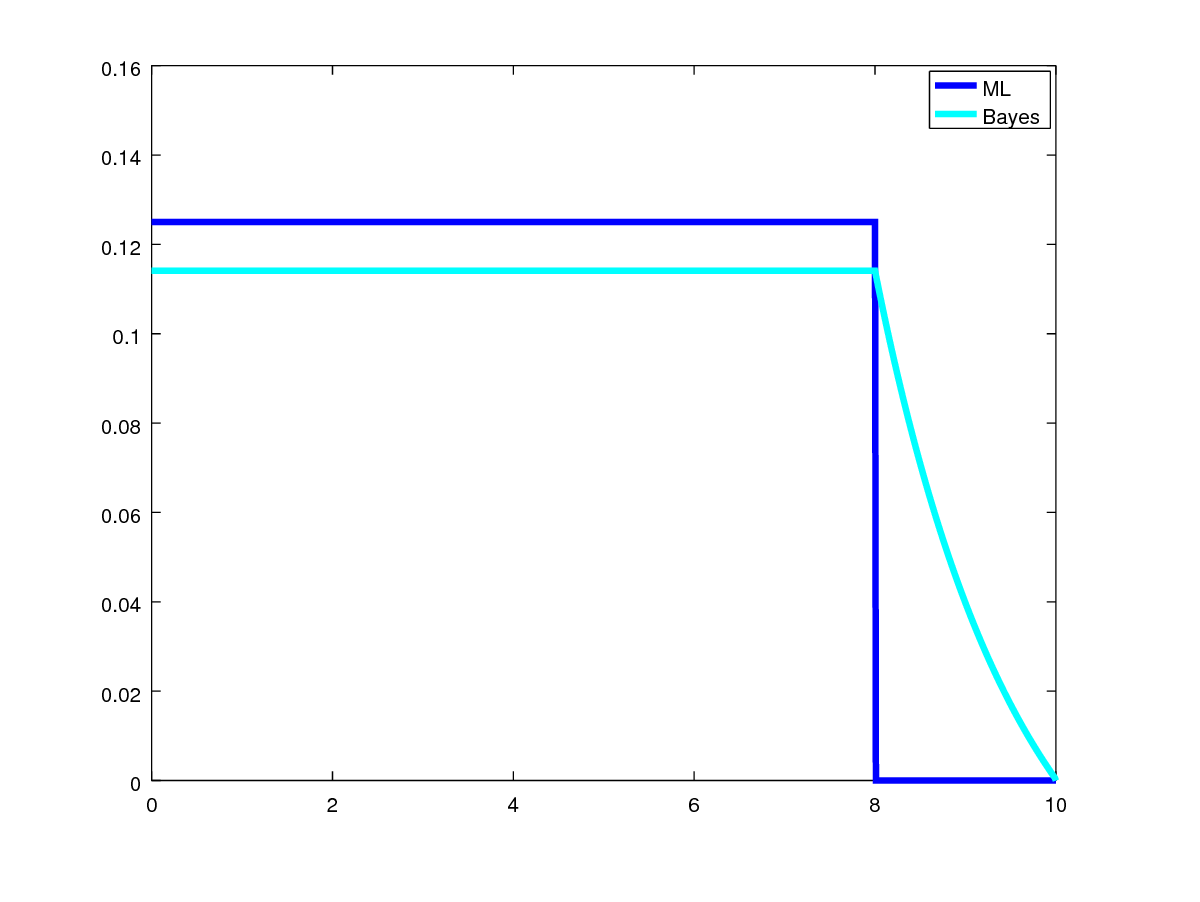
\includegraphics[width=0.5\textheight]{Question2_2.png}
	\end{enumerate}
	\section{Principal Component Analysis}
	\begin{enumerate}
		\item [(a)]Determine the scatter matrix \\
		Ans : \\
		\[mean=\frac{1}{30}\sum_{k=1}^{30}x_k=\left[
		\begin{array}{clr}0.0304 \\ 0.0418 \\ -0.0762\end{array} \right] \]
		\[S=\sum_{k=1}^{n}(x_k-m)(x_k-m)^t \]
		\[s=\left[
		\begin{array}{clr}13.5236 & 10.3097 & 4.6601 \\ 10.3097 & 55.2695 & 13.0659 \\ 4.6601 & 13.0659 & 70.8436\end{array} \right] \]
		\item [(b)]Determine the two largest eigenvalues of the scatter matrix and the corresponding eigenvectors.
		Ans: \\
		criterion function : \[J(x_0)=\sum_{k=1}^{n}\Vert x_0-x_k\Vert^2 \]
		\[a_k=e^t(x_k-m) \qquad x_0=\frac{1}{n}\sum_{k=1}^{n}x_k=m+ae\]
		\[J(e)=\sum_{k=1}^{n}\Vert(m+a_ke)-x_k\Vert^2 \]
		\[=\sum_{k=1}^{n}\Vert a_ke-(x_k-m)\Vert^2 \]
		\[=\sum_{k=1}^{n}a_k^2\Vert e\Vert^2-2\sum_{k=1}^{n}a_ke^t(x_k-m)+\sum_{k=1}^{n}\Vert x_k-m\Vert^2 \]
		\[=-\sum_{k=1}^{n}[e^t(x_k-m)]^2+\sum_{k=1}^{n}\Vert X_k-m\Vert^2 \]
		\[=-\sum_{k=1}^{n}e^t(x_k-m)(x_k-m)^te+\sum_{k=1}^{n}\Vert x_k-m\Vert^2 \]
		\[=-e^tSe+\sum_{k=1}^{n}\Vert x_k-m\Vert^2 \]
		\[Assume :\Vert e\Vert^2=1 \]
		\[Se=\lambda e\quad ,e^tSe=\lambda e^te=\lambda \]
		\[eigen\ vector=\left[\begin{array}{clr}0.1710 & 0.1400 \\ 0.8290 & 0.5145 \\ -0.5324 &  0.8460\end{array} \right]\]
		\[eigen\ value=\left[\begin{array}{clr}49.0038 & 79.5607\end{array} \right] \]
		\item [(c)]Plot the projected data points on the two-dimensional subspace \\
		 Ans:\\
			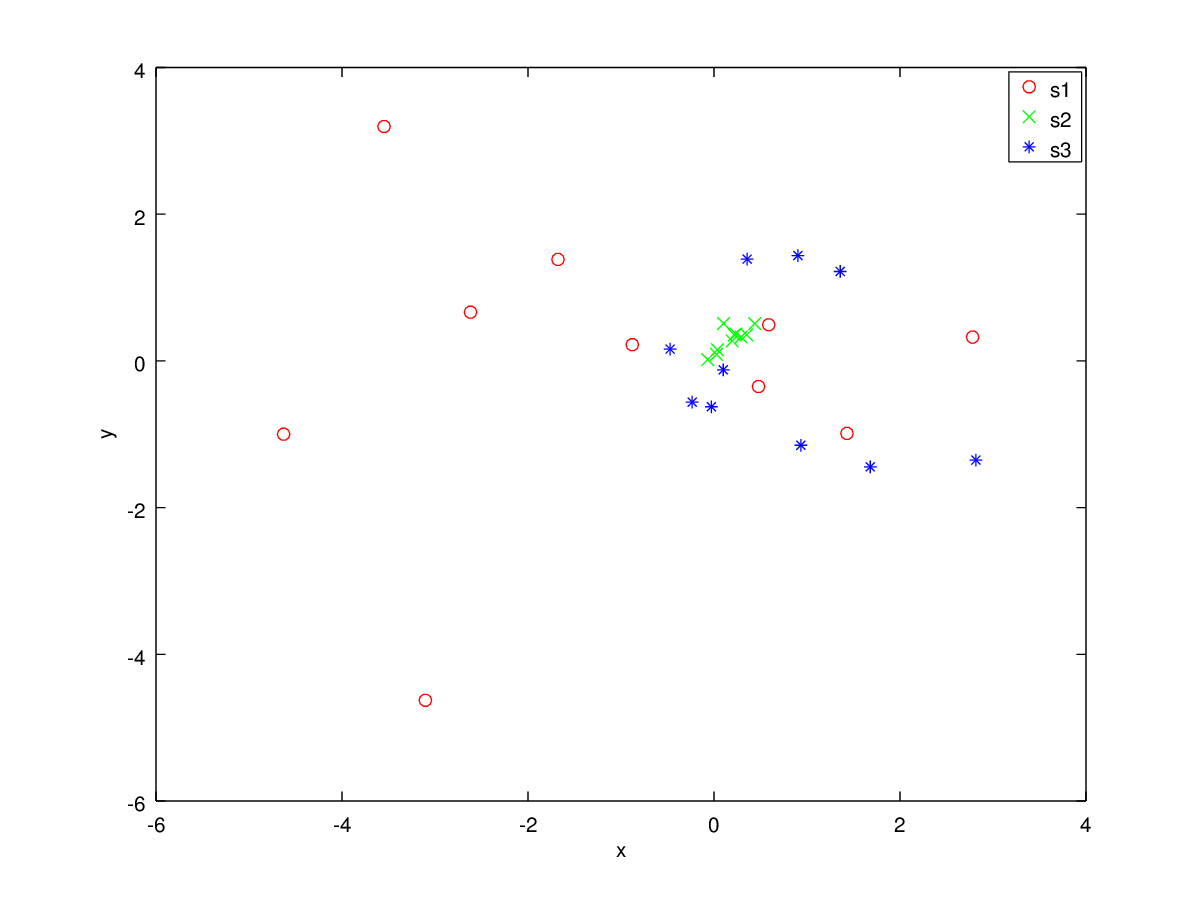
\includegraphics[width=0.5\textheight]{Question3.png}
		\item[(d)]Assume that the prior probabilities are equal and the class-conditional
		probability density functions are normal. Calculate the percentage of
		misclassified samples in the two-dimensional subspace 
		Ans : \\
		\[Error\ rate=\frac{1-correct\ sample}{total\ sample} \]
		\[e_1=0.5\qquad e_2=0\qquad e_3=0 \]
		
	\end{enumerate}
	\section{Fisher Linear Discriminant}
	\begin{enumerate}
		\item [(a)]Determine the within-class scatter matrix $S_W$ and the between-class
		scatter matrix $S_B$ \\
		Ans : \\
		\[S_i=\sum_{x\in D_i}^{c}(x-m_i)(x-m_i)^t \]
		\[S_w=\sum_{i=1}^{c}S_i \]
		\[s_1= \left[\begin{array}{clr}9.0618 & 5.6778 & 3.9408 \\ 5.6678 & 42.0071 & 7.3370 \\ 3.9408 & 7.3370 & 45.4195\end{array} \right] \]
		\[s_2= \left[\begin{array}{clr}0.5393 & -0.1465 & -0.0518 \\ -0.1465 & 0.4597 & 0.0851 \\ -0.0518 & 0.0851 & 0.0727\end{array} \right] \]
		\[s_3= \left[\begin{array}{clr}3.0186 & 4.0474 & -1.8042 \\ 4.4074 & 6.4496 & -2.0130 \\ -1.8042 & -2.0130 & 12.6214\end{array} \right] \]
		\[s_w= \left[\begin{array}{clr}12.6196 & 9.5787 & 2.0848 \\ 9.5787 & 48.9165 & 5.4091 \\ 2.0848 & 5.4091 & 58.1136\end{array} \right] \]
		\[S_{Bi}=n_i(m_i-m)(m_i-m)^t \]
		\[S_B=S_{B1}+S_{B2}+S_{B3} \]
		\[m_i=\frac{1}{10}\sum_{k=1}^{10}x_{ki}\quad, n_i=number\ of \ sample\quad, m=\sum_{i=1}^{3}m_i \]
		\[S_{B1}=\left[\begin{array}{clr}0.1026 & 0.6549 & 0.8456 \\ 0.6549 & 4.1792 & 5.3965 \\ 0.8456 & 5.3965 & 6.9685\end{array} \right] \]
		\[S_{B2}=\left[\begin{array}{clr}0.2045 & -0.5550 & -0.1143 \\ -0.5550 & 1.5065 & 0.3103 \\ -0.1143 & 0.3103 & 0.0639\end{array} \right] \]
		\[S_{B3}=\left[\begin{array}{clr}0.5968 & 0.6311 & 1.8440 \\ 0.6311 & 0.6674 & 1.9500 \\ 1.8440 & 1.9500 & 5.6976\end{array} \right] \]
		\[S_{B}=\left[\begin{array}{clr}0.9039 & 0.7309 & 2.5753 \\ 0.7309 & 6.3530 & 7.6568 \\ 2.5753 & 7.6568 & 12.7300\end{array} \right] \]
		\item [(b)](b) Determine the two largest eigenvalues of 𝑆𝑊−1𝑆𝐵 and the corresponding
		eigenvectors. \\
		Ans : \\
		\[Assume\ f(w)=w^TS_Bw\ ,st\ g(w)=w^TS_ww=c \]
		\[\frac{\partial}{\partial w}[f(w)-\lambda(g(w)-c)]=0 \]
		\[\frac{\partial}{\partial w}[w^TS_Bw-\lambda(w^TS_Bw-c)]=(S_B+S_B^T)w-\lambda(S_w+S_w^T)=0 \]
		\[S_Bw=\lambda S_ww \]
		\[S_w^{-1}S_Bw=\lambda S_ww=\lambda w \]
		\[\max J(w)=\frac{w^TS_Bw}{w^TS_ww}=\lambda_{max}=v_{max}=\left[\begin{array}{clr}0.1386 & -0.9081 \\ 0.5653 & 0.4046 \\0.8132 & -0.1079\end{array} \right] \]
		\[Eigenvalues=\left[\begin{array}{clr}0.2972 & 0 \\ 0 & 0.1028 \\ 0 & 0\end{array} \right] \]
		\item [(c)]Plot the projected data points on the two-dimensional subspace.\\
		Ans :\\
		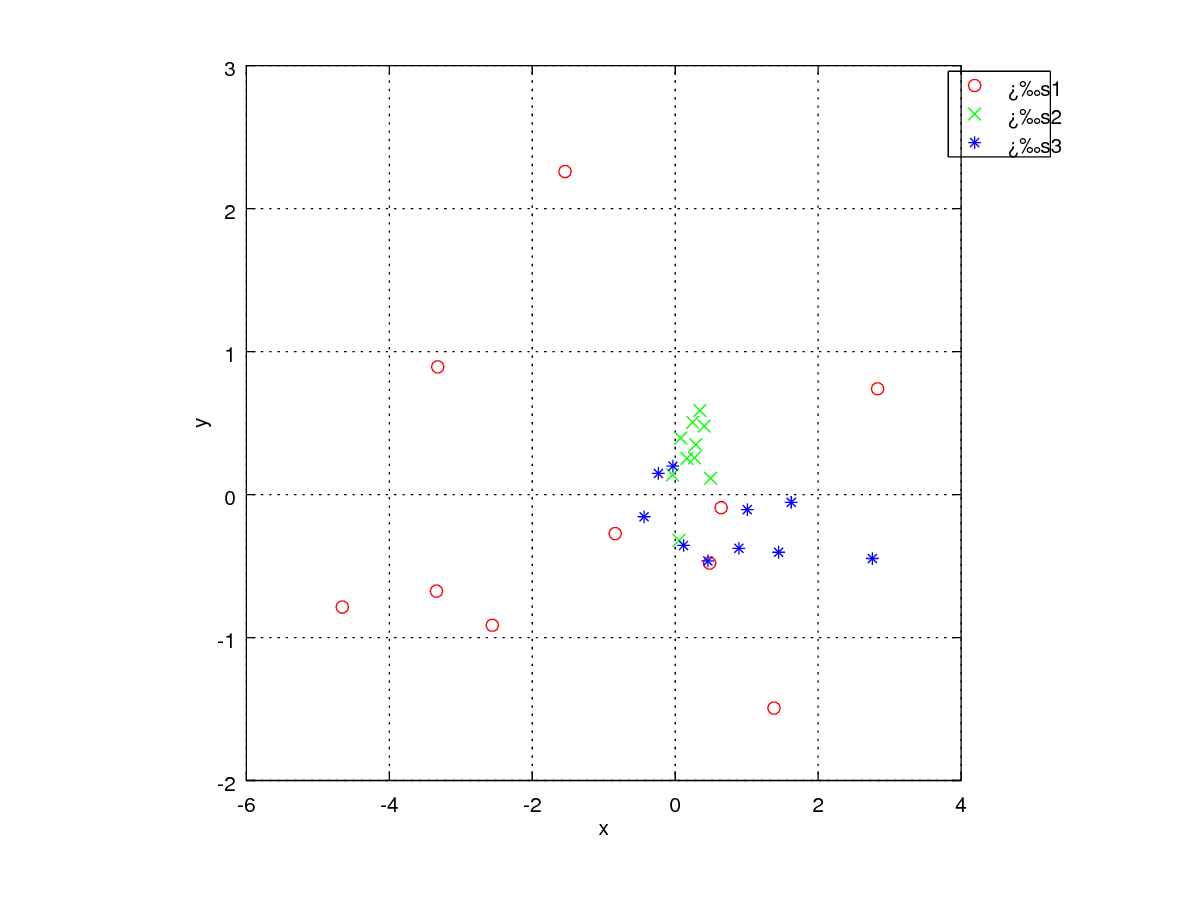
\includegraphics[width=0.5\textheight]{Question4.png}
		
		\item [(d)]Assume that the prior probabilities are equal and the class-conditional
		probability density functions are normal. Calculate the percentage of
		misclassified samples in the two-dimensional subspace. \\
		Ans : \\
		\[Error\ rate=\frac{1-correct\ sample}{total\ sample} \]
		\[e_1=0.3\qquad e_2=0.1\qquad e_3=0.1 \]
	\end{enumerate}


	
	
\end{document} 